\documentclass[a4paper,14pt,russian]{article}
\usepackage{./coursework}
\usepackage{titlesec}
\usepackage[export]{adjustbox}
\usepackage{lastpage}
\newcommand{\caphedre}{ВТ}
\newcommand{\theme}{Проектирование локальной вычислительной сети}
\newcommand{\groupnumber}{5305}
\newcommand{\studentname}{Билькис П.П.}
\newcommand{\teachername}{Белова Е.Ю.}
\newcommand{\discipline}{Сети ЭВМ}
\newcommand{\myyear}{2018}
\begin{document}

\begin{titlepage}

\thispagestyle{empty}

\centerline{МИНОБРНАУКИ РОССИИ}
\centerline{САНКТ-ПЕТЕРБУРГСКИЙ ГОСУДАРСТВЕННЫЙ}
\centerline{ЭЛЕКТРОТЕХНИЧЕСКИЙ УНИВЕРСИТЕТ}
\centerline{<<ЛЭТИ>> ИМ. В.И. УЛЬЯНОВА (ЛЕНИНА)}
\centerline{Кафедра \caphedre}

\vfill

\centerline{\large{\textsc{КУРСОВОЙ ПРОЕКТ}}}
\centerline{\large{по дисциплине <<\discipline>>}}
\centerline{\large{Тема: \theme}}

\vfill

Студент группы \groupnumber \hfill \studentname

Преподаватель \hfill \teachername

\vfill

\centerline{Санкт-Петербург}
\centerline{\myyear}
\clearpage
\end{titlepage}
\setcounter{page}{2}

\section*{Задание на курсовой проект}

Студент \studentname\\
Группа \groupnumber\\\\
Тема работы: \theme\\
Исходные данные:\\
Профиль организации, количество зданий, количество этажей в каждом здании, минимальное количество сотрудников, минимальное количество серверов.
Содержание пояснительной записки:\\
«Аннотация», «Содержание», «Введение», «Описание организации», «Разработка транспортной подсистемы локальной вычислительной сети», «Расчет стоимости локальной вычислительной сети», «Список использованных источников», «Заключение», «Приложения».
Предполагаемый объем пояснительной записки:\\
Не менее \pageref{LastPage}
Дата выдачи задания: 01.02.2018\\
Дата сдачи реферата: 17.05.2018\\
Дата защиты реферата: 17.05.2018\\

\vfill


Студент группы \groupnumber \hfill \studentname


Преподаватель \hfill \teachername


\clearpage

\selectlanguage{russian}
\begin{abstract}
  В курсовом проекте необходимо выполнить проектирование локальной вычислительной сети производства одежды. В первой части проекта приведено описание функций и структуры производства, направлений работы его подразделений. Вторая часть проекта включает в себя разработку транспортной подсистемы локальной вычислительной сети производства одежды. В третьей части проекта выполнена оценка стоимости локальной вычислительной сети и её дальнейшая эксплуатация, выдвинуты требования к составу обслуживающего персонала.
\end{abstract}


\selectlanguage{english}
\begin{abstract}
  In this coursework local computer network for the clothes manufacture is described. The first section presented basic stucture \& functions of the manufacture, it's subdivisions and their responsibilities are depicted. The second, however, describes transport sub-system of the local computer network. The third section contains of cost estimations for bulding and supporting this local computer network, and staff requirements.
\end{abstract}

\clearpage

\selectlanguage{russian}
\tableofcontents
\clearpage

\section*{Введение}
\addcontentsline{toc}{section}{Введение}
Данный курсовой проект предусматривает создание локальной вычислительной сети для производства одежды. Осуществляется это с помощью первичного проектирования планировки здания учреждения с последующей установкой необходимых устройств коммутации и их настройки.
\clearpage

\section{Описание организации}

\subsection{Функции организации}
% Функции организации
В рамках курсового проекта разрабатывается корпоративная сеть для производства одежды. Продукция производства - мужская и женская одежда, широкий спектр: от нижнего белья до верхней одежды из кожи.
Производство представляет из себя Закрытое Акционерное Общество (ЗАО).1

\subsection{Структура организации и функции подразделений}
% Структура организации и функции подразделений
Предприятие состоит из Административной части, Основного производства и Вспомогательного производства.

\subsubsection{Административная часть}
Административная часть состоит из следующих подразделений:
\begin{description}
\item [Отдел кадров]
  Отдел осуществляет контроль за текущей потребностью в кадрах, составляет списки резерва кадров, учувствует в работе по отбору кандидатов на работу, ведёт учет личного состава, оформляет документы о приеме сотрудников на работу, ведёт установленную документацию по кадрам.
\item [Отдел закупок]
  Отдел осуществляет поиск, анализ данных, выбор поставщиков необходимого оборудования. Проверяет поступающую продукцию.
\item [Отдел продаж]
  Отдел осуществляет рекламную деятельность, направленную на увеличение продаж продукции. Производит работу с клиентами, направленную на поддержание связей и увеличения объёмов взаимного сотрудничества.
\item [Отдел технического обеспечения]
  Отдел осуществляет ремонт или заменую сломанного оборудования.
\item [Бухгалтерия]
  Бухгалтерия занимается ведением бухгалтерского, налогового и управленческого учета финансово-хозяйственной деятельности завода, формирует бухгалтерскую, налоговую и управленческую отчетность, взаимодействует с государственными налоговыми органами, взаимодействует с финансовыми организациями в пределах своей компетенции, осуществляет платежи.
\item [IT-отдел]
  Отдел обеспечивает работоспособность локальной компьютерной сети, серверов и рабочих станций пользователей, обеспечивает информационную безопасность, антивирусную защиту, проводит техническое обслуживание и организацию ремонта вычислительной и оргтехники, обеспечивает рабочие станции и сервера свободным программным обеспечением.
\item [Хозяйственный отдел]
  Отдел обеспечивает хозяйственное, материально-техническое и социально-бытовое обслуживание издательства, контролирует исправность оборудования (лифтов, освещения, систем отопления и др.), оформляет документы, необходимые для заключения договоров на приобретение оборудования, обеспечивает подразделения канцелярскими принадлежностями, оборудованием, оргтехникой, мебелью, хозяйственными товарами, обеспечивает сохранность вышеуказанного оборудования, оформляет документы на техническое обслуживание и ремонт оргтехники и оборудования, занимается содержанием в надлежащем состоянии зданий и помещений предприятия.
\end{description}

\subsubsection{Основное производство}
\begin{description}
\item [Цех по пошиву лёгкого женского платья]
  Цех занимается пошивом лёгкого женского платья из готовых раскроек.
\item [Цех по пошиву головных уборов]
  Цех занимается пошивом головных уборов из готовых раскроек.
\item [Цех по пошиву женской верхней одежды]
  Цех занимается пошивом женской верхней одежды из готовых раскроек.
\item [Цех по пошиву мужской верхней одежды]
  Цех занимается пошивом мужской верхней одежды из готовых раскроек.
\item [Цех по пошиву изделий из кожи]
  Цех занимается пошивом и раскройкой изделий из кожи.
\item [Раскройный цех]
  Цех готовит раскройки для пошива изделий во всех пошивных цехах (кроме цеха по пошиву изделий из кожи).
\item [Экспериментальный цех]
  В экспериментальном цеху проходят апробацию новейшие технологии, методы, оборудования и приёмы для изготовления одежды.
\end{description}
\subsubsection{Вспомогательное производство}
\begin{description}
\item [Ремонтно-механический цех]
  Ремонтно-механический цех занимается текущим ремонтом и обслуживанием оборудования производства.
\end{description}

\section{Разработка транспортной подсистемы локальной вычислительной сети}

\subsection{Описание поэтажных планов зданий организации}
% Описание поэтажных планов зданий организации
\begin{description}
\item [1-е здание]
  Двухэтажное.
  \begin{description} 
  \item[1-й этаж]
  Отдел кадров (20 человек), отдел закупок (15 человек).
\item[2-й этаж]
  Отдел продаж (15 человек), бухгалтерия (20 человек).
\end{description}
Нумерация кабинетов слева направо по часовой стрелке, начиная с 1100 и заканчивая 1204. Вторая цифра обозначает этаж. В кабинетах с 1100 по 1103 размещаются сотрудники отдела кадров, в кабинетах с 1104 по 1106 размещаются сотрудники отдела закупок, в кабинетах с 1200 по 1202 размещаются сотрудники отдела продаж, в кабинетах с 1203 по 1206 располагается бухгалтерия. В каждом кабинете по 5 рабочих мест. Положение информационных розеток указано на плане. В помещении 1107 располагается стойка с сетевым оборудованием.
\item [2-е здание]
  Двухэтажное.
  \begin{description}
\item [1-й этаж]
  Отдел технического обеспечения (10 человек), хозяйственный отдел (15 человек).
\item[2-й этаж]
  IT-отдел (5 человек).
\end{description}
  Нумерация кабинетов слева направо по часовой стрелке, начиная с 2100 и заканчивая 2202. Вторая цифра обозначает этаж. В кабинетах с 2100 по 2101 размещаются сотрудники отдела технического обеспечения, в кабинетах с 2102 по 2103 размещаются сотрудники хозяйственного отдела, а в кабинетах с 2200 по 2201 размещаются IT-отдел.
  В кабинете 2102 10 рабочих мест, в остальных кабинетах по 5 рабочих мест. Положение информационных розеток указано на плане. В помещении 2202 располагается стойка с сетевым оборудованием.
\item [3-е здание]
  Двухэтажное.
 \begin{description} 
 \item[1-й этаж]
  Цех по пошиву женской верхней одежды (20 человек).
  \item[2-й этаж]
  Цех по пошиву лёгкого женского платья (15 человек).
\end{description}
  Оба цеха представляют собой помещения без деления на кабинеты. В каждом цеху есть потребнось в пяти компьютезированных рабочих местах, подключённых к  локальной вычислительной сети.
  
\item [4-е здание]
  Одноэтажное.\\
  В здании располагается цех по пошиву мужской верхней одежды - 10 человек.
  Цех представляет собой помещение без деления на кабинеты, занимает весь этаж. В цеху есть потребность в пяти компьютезированных рабочих местах, подключённых к локальной вычислительной сети.
\item [5-е здание]
  Одноэтажное.\\
  В здании располагается склад материалов и готовой продукции. Склад делится на два помещения, в одном располагается склад материалов, во втором - готовой продукции. В каждом помещении работает по 10 человек, имеется по 5 рабочих мест, подключённых к ЛВС.
\end{description}

\subsection{Выбор топологии локальной вычислительной сети}
% Выбор топологии локальной вычислительной сети

\subsection{Соединение удалённого коммуникационного оборудования}
% Соединение удалённого коммуникационного оборудования
Для соединения коммутационного оборудования, которое находятся в различных зданиях, кабель витая пара чаще всего не используется, поэтому целесообразно рассмотреть две технологии: VPN и волокно-оптические системы связи.
VPN (Virtual Private Networks – Виртуальные частные сети) технология используется при объединении нескольких сетей, в одну виртуальную сеть, позволяя пользователям использовать ресурсы сетей всех офисов компании, как единую сеть. Отличное VPN сети от локальной сети состоит в том, что в VPN для передачи данных используется опорные сети оператора и Интернет каналы, а не кабель витой пары. Вся передаваемая по VPN информация надежно шифруется. 
Волокно-оптическая система связи (ВОЛС) – это вид системы передачи, при котором информация передается по оптическим диэлектрическим волноводам, известным под названием оптическое волокно. ВОЛС используется при построении объектов, в которых СКС должна объединить многоэтажное здание или при объединении территориально-разрозненных зданий. Оптически кабель может быть многомодовым (обеспечивает передачу сигналов на расстояние 1-5 км) и одномодовым (обеспечивает передачу сигналов на расстояние в десятки километров). Скорость передачи данных по оптоволокну ограничивается только пропускной способностью передающего и приемного модуля системы. Как правило, передача данных по оптоволокну составляет от 1 до 10 Гбит/с. Поэтому оптоволоконные системы чаще всего используется для передачи больших объемов информации, в том числе аудио и видеосигналов.
В рамках курсового проекта выбрана ВОЛС, поскольку её целесообразно использовать для соединения коммутационного оборудования, которое расположено в пределах километра друг от друга. Для прокладки ВОЛС применяется подземный метод, суть которого заключается в осуществлении монтажа кабеля по подземным коммуникациям. Данный метод позволяет оградить ВОЛС от нежелательных повреждений и негативного воздействия окружающей среды.
Для соединения двух удаленных маршрутизаторов друг с другом, необходимо наличие модулей SFP. Данные модули используются для присоединения платы маршрутизатора к ВОЛС.

\subsection{Выбор серверного оборудования}
% Выбор серверного оборудования
К коммутатору 3 уровня, который находится в главной серверной (монтажный шкаф 3) будут подключены следующие сервера:
\begin{description}
\item[Файловый сервер]
  Данный сервер представляет собой компьютер, первичной целью которого является обеспечение доступа к файлам (таких как документы, звуковые файлы, фотографии, изображения и т.д.), размещенных на его устройствах хранения информации, другим компьютерам издательства. Плюсами использования сервера являются: экономия пространства жесткого диска персональных компьютеров, обеспечение совместной работы пользователей с информационными ресурсами, надежность хранения информации. Сервер в локальной сети использует протокол SMB/CIFS (Windows и Unix-подобные операционные системы). Клиенты соединяются с сервером, используя протоколы TCP. После того, как соединение установлено, клиенты могут посылать команды серверу (эти команды называются SMB-команды), который дает им доступ к ресурсам, позволяет открывать, читать файлы, писать в файлы и, вообще, выполнять весь перечень действий, которые можно выполнять с файловой системой. В случае SMB, данные действия совершаются через сеть.

\item[Сервер печати]
  Он обеспечивает совместный доступ к принтеру, подключённому к серверу для определённого списка машин локальной сети.
\item[Сервер электронной почты]
  Сервер обеспечивает:
  \begin{itemize}
  \item Прием электронной почты завода из Интернет и ее раскладку по отдельным ящикам внутри общего домена
  \item Проверку входящей почты на наличие вирусов и их обезвреживание в случае необходимости
  \end{itemize}
  Размеры почтовых ящиков пользователей ограничены только возможностями сервера. На сервере организован электронный документооборот и обмен сообщениями внутри издательства. Вся конфиденциальная информация остается в пределах локальной сети.
  Когда пользователь набрал сообщение и посылает его получателю, почтовый клиент взаимодействует с почтовым сервером, используя протокол SMTP. Почтовый сервер отправителя взаимодействует с почтовым сервером получателя. На почтовом сервере получателя сообщение попадает в почтовый ящик, откуда при помощи агента доставки сообщений (MDA) доставляется клиенту получателя. Для финальной доставки полученных сообщений используется протокол POP3 или IMAP.
\item[Сервер баз данных]
  Сервер БД обслуживает базу данных и отвечает за целостность и сохранность данных, а также обеспечивает операции ввода-вывода при доступе к информации. Применяемая база данных – MySQL. В базе данных содержится полная информация о перечне часов, выпускаемых заводом.
\item[Веб-сервер]
  Данный сервер обеспечивает размещение и выдачу по запросу любой информации в формате HTML, что позволяет издательству организовать собственное Интернет представительство, прорекламировать свои услуги и продукты, довести до конечных пользователей прейскурант, получить обратную связь.
  Клиент, которым обычно является веб-браузер, передаёт веб-серверу запросы на получение ресурсов, обозначенных URL-адресами. Ресурсы – это HTML-страницы, изображения, файлы, медиа-потоки или другие данные, которые необходимы клиенту. В ответ веб-сервер передаёт клиенту запрошенные данные. Такой обмен происходит по протоколу HTTP.
\item[Сервер резервного копирования файлов]
  Сервер производит копирование наиболее ценной информации на магнитную ленту или магнитооптические диски. Если какой-либо из серверов полностью вышел из строя или вся база данных была случайно удалена, сервер резервного копирования становиться незаменимым. Сервер резервного копирования может некорректно сохранить некоторые данные (например, сообщения с почтового сервера). Чтобы этого не происходило, существуют программы-агенты для каждого из сетевых приложений. Они поставляются как дополнение к серверу резервного копирования.
\item[Прокси-сервер]
  Данный сервер действует как посредник, помогая пользователям получить информацию из Интернета (трансляция запросов к WWW и FTP ресурсам) и при этом, обеспечивая защиту сети, может сохранять часто запрашиваемую информацию в кэш-памяти на локальном диске, быстро доставляя её пользователям без повторного обращения к Интернету, делая потребление Интернет трафика более экономичным. Кроме того, он может вводить ограничение доступа к ресурсам Интернет для рабочих станций локальной сети в соответствии с внутрикорпоративной политикой безопасности.
  Прокси-сервер сконфигурирован таким образом, что принимает или отвергает определённые типы сетевых запросов, поступающие как из локальной сети, так и из Интернета. В такой конфигурации прокси-сервер становиться межсетевым экраном – брандмауэром. Он обеспечивает:
  \begin{itemize}
  \item Защиту локальной сети предприятия от несанкционированного и неправомерного доступа из сети Интернет к ресурсам локальной сети организации;
  \item Трансляцию внутренних адресов локальной сети в публичные Интернет адреса (NAT – network address translation);
  \item Ограничение доступа в Интернет машин локальной сети (Proxy, ACL);
  \item Ограничение ресурсов сети Интернет для доступа из локальной сети (возможно разграничение доступа к серверам WWW в зависимости от содержания).
  \end{itemize}
\end{description}

\subsection{Адресация}
% Выбор коммутационного оборудования

\subsection{Выбор оборудования}
% Выбор коммутационного оборудования

\section{Расчёт стоимости и эксплуатации локальной вычислительной сети}

\subsection{Расчёт стоимости оборудования и комплектующих}
% Расчёт стоимости оборудования и комплектующих
\begin{table}[!htbp]
  \centering
  \begin{tabular}{|p{3cm}|p{2cm}|p{2cm}|}
    \hline
    Наименование & Количество & Итоговая стоимость \\ \hline
    Коммутатор 2-го уровня 24 порта & 11 & \\ \hline
    Коммутатор 3-го уровня 8 портов & 5 & \\ \hline
    Витая пара & 1488 метров & \\ \hline
    Патч-корд & & \\ \hline
    Информационная розетка (однопортовая) & & \\ \hline
    Информационная розетка (двупортовая) & & \\ \hline
    Патч-панель 24 порта & 3 & \\ \hline
    Патч-панель 48 портов & 4 & \\ \hline
    Гофротруба & 300 метров & \\ \hline
    Кабель-канал & 1500 метров & \\ \hline
    Оптоволоконный кабель & 200 метров & \\ \hline
    SFP-модуль & 8 & \\ \hline
    Сервера & 11 & \\ \hline
    Монтажные шкафы (настенные) & 8 & 35920 \\ \hline
    Монтажные шкафы (напольные) & 1 & 40070 \\ \hline
    ИБП & 5 & \\ \hline
    \textbf{Итого:} & & \\ \hline
  \end{tabular}
  \caption{Итоговая стоимость оборудования}
  \label{table:cabel}
\end{table}

\subsection{Расчёт стоимости эксплуатации}
% Расчёт стоимости эксплуатации

\subsection{Требования к составу обслуживающего персонала}
% Требования к составу обслуживающего персонала
IT-отдел должен быть укомплектован двумя системными администраторами для поддержания сети в рабочем состоянии и дальнейшего её развития, а так же тремя специалистами IT-поддержки.

\begin{description}
\item[Специалист IT-поддержки] Данный специалист нацелен на помощь конечным пользователям и решение их компьютерных проблем.\\
  Обязанности:
  \begin{itemize}
  \item Работа на первой линии техподдержки. Обработка заявок от сотрудников, ответ на звонки, устранение технических неисправностей. 
  \item Настройка и администрирование рабочих станций, установка и настройка ПО
  \item Администрирование сети, обеспечение бесперебойной работы сетевого оборудования
  \item Поддержка и настройка IP телефонии
  \item Администрирование 1С Предприятие
  \item Тестирование и ремонт ПК
  \item Обеспечение работы копировальной техники
  \item Организация новых рабочих мест
  \item Инвентаризация ПО и оборудования
  \end{itemize}

  Заработная плата: 30000р/месяц\\
  Количество сотрудников: 3.
\item[Системный администратор] Данный специалист должен поддерживать сеть в рабочем состоянии. \\
  Обязанности:
  \begin{itemize}
  \item Администрирование сети, обеспечение бесперебойной работы сетевого оборудования
  \item Администрирование серверов под управлением ОС GNU/Linux
  \item Инвентаризация ПО и оборудования
  \item Настройка новой техники, оборудования
  \end{itemize}
  Заработная плата: 45000р/месяц\\
  Количество сотрудников: 2.
\end{description}

Итого затраты: 180000р/месяц



\section*{Заключение}
\addcontentsline{toc}{section}{Заключение}
В процессе курсового проекта была спроектирована локальная сеть, построены поэтажные планы и планы корпусов. Так же были посчитаны длины кабелей, затраты на покупку и обслуживание оборудования, выдвинуты требования к обслуживающему персоналу.

\renewcommand\refname{Список использованных источников}
\nocite{*}
\bibliographystyle{./utf8gost705u}
\bibliography{biblio}
\appendix
\section{Поэтажный план здания №1}
\begin{figure}
  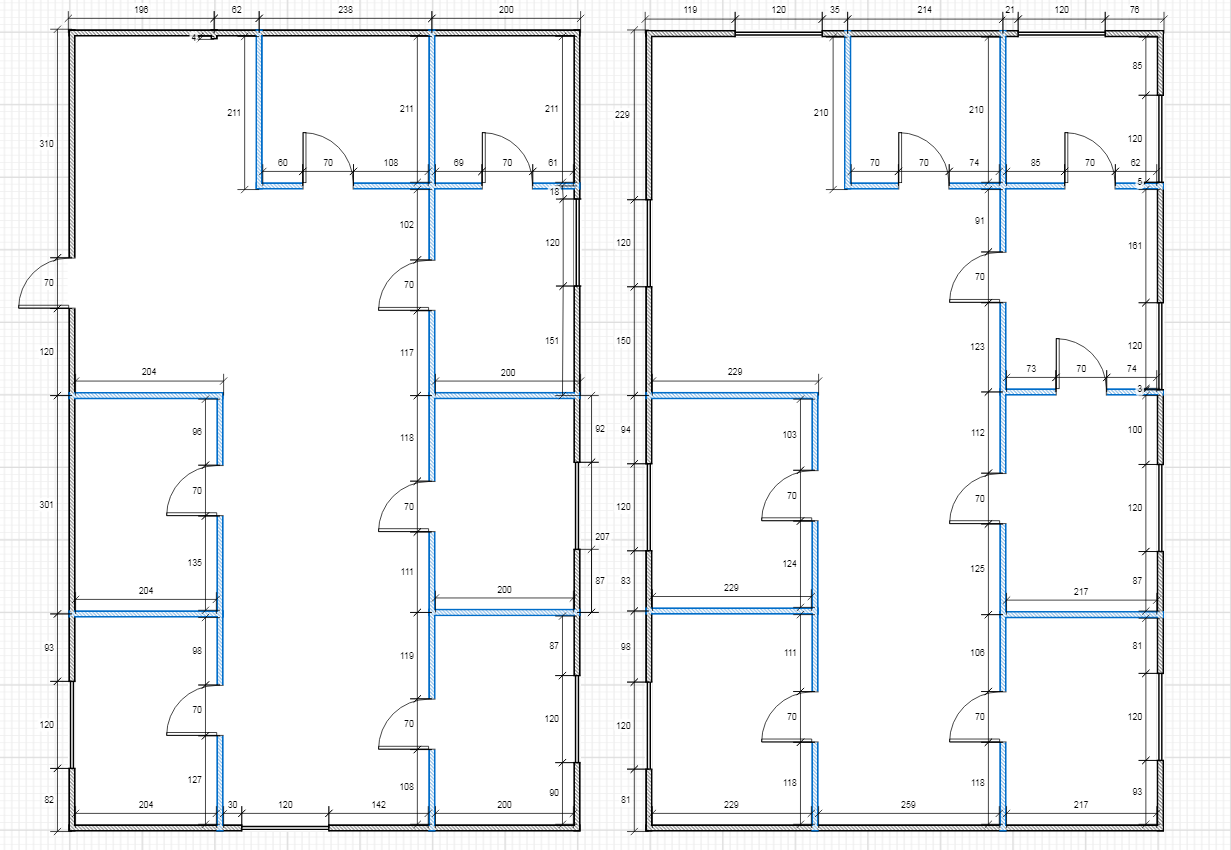
\includegraphics[scale=0.58]{./1-building.png}
 \caption{Поэтажный план здания №1}
\end{figure}
\section{Поэтажный план здания №2}
\begin{figure}
  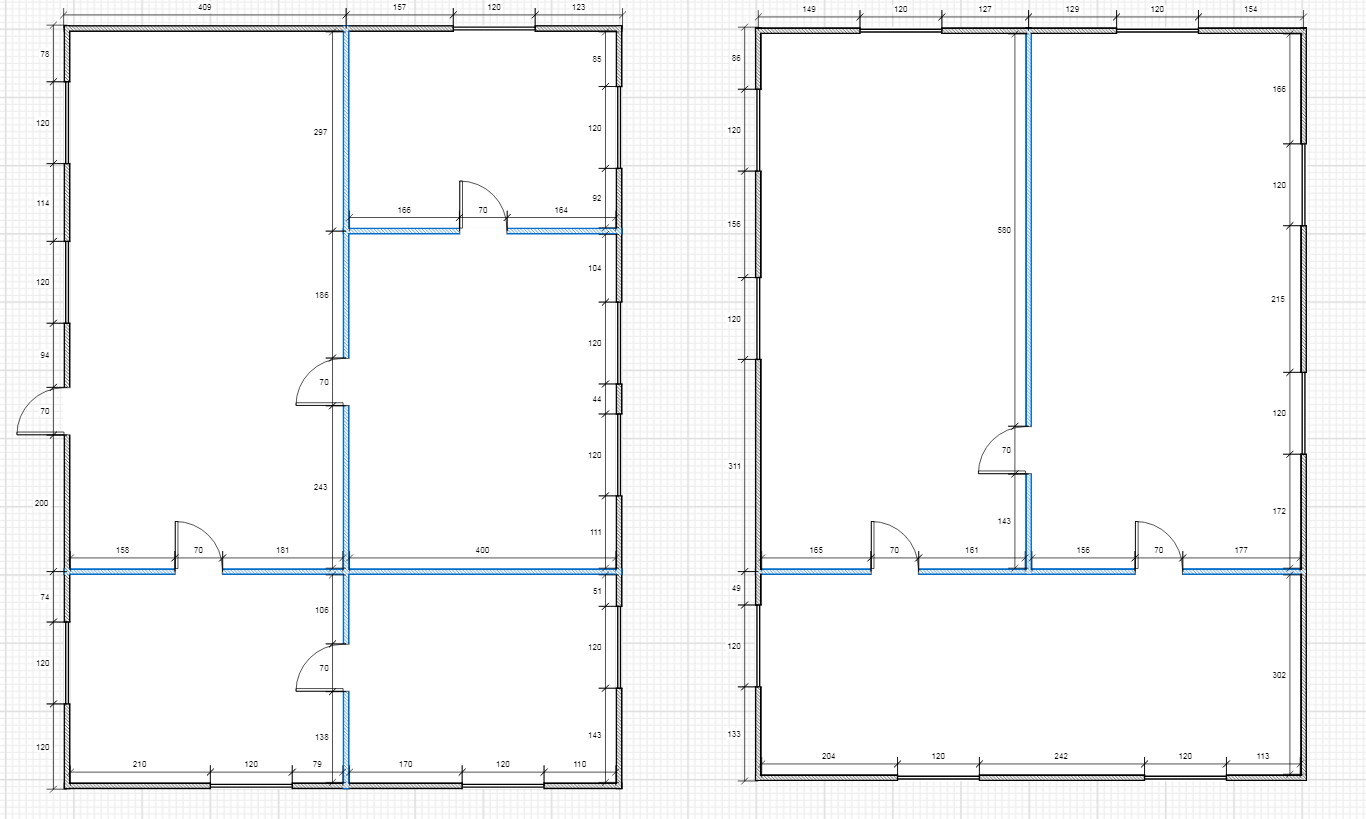
\includegraphics[scale=0.50]{./2-building.png}
 \caption{Поэтажный план здания №2}
\end{figure}
\section{Поэтажный план здания №3}
\begin{figure}
  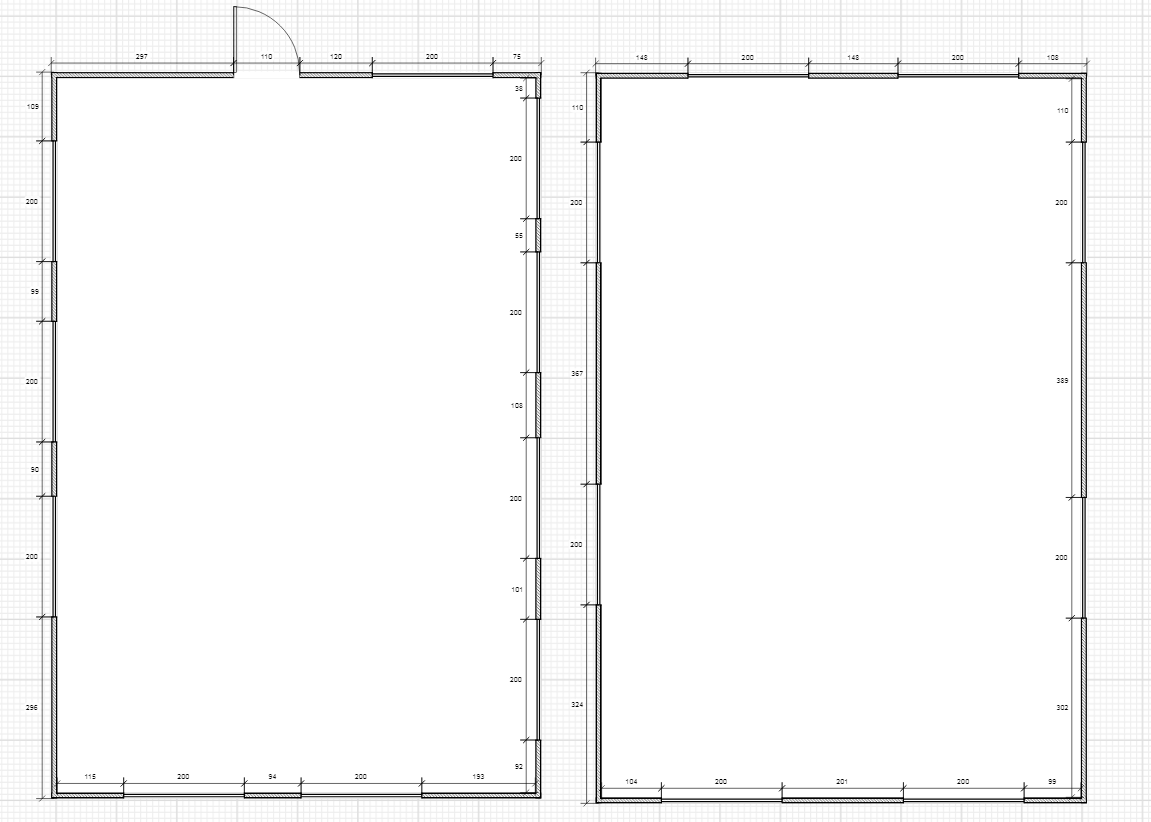
\includegraphics[scale=0.58]{./3-building.png}
 \caption{Поэтажный план здания №3}
\end{figure}
\section{Поэтажный план здания №4}
\begin{figure}
  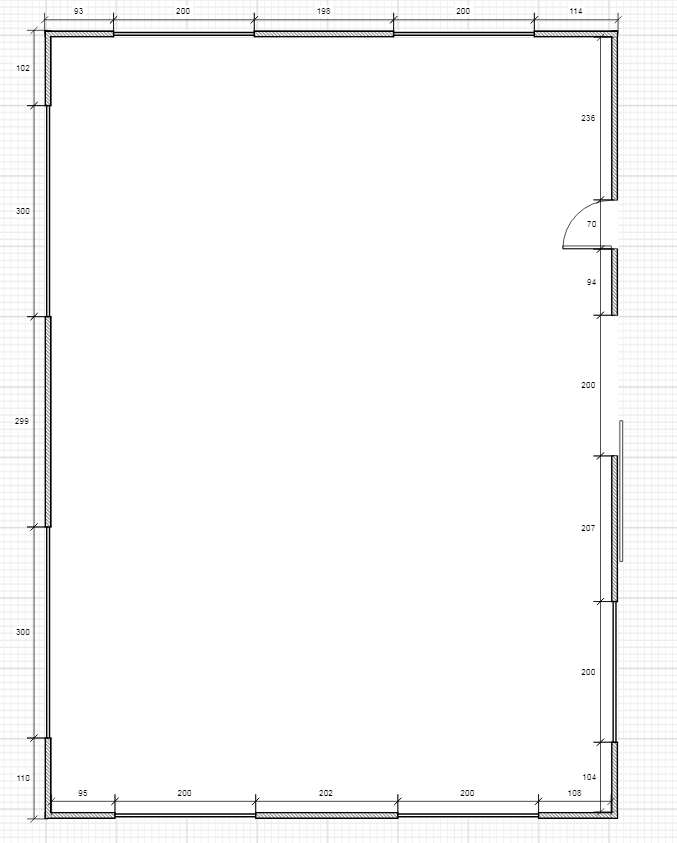
\includegraphics[scale=0.58]{./4-building.png}
 \caption{Поэтажный план здания №4}
\end{figure}
\section{Поэтажный план здания №5}
\begin{figure}
  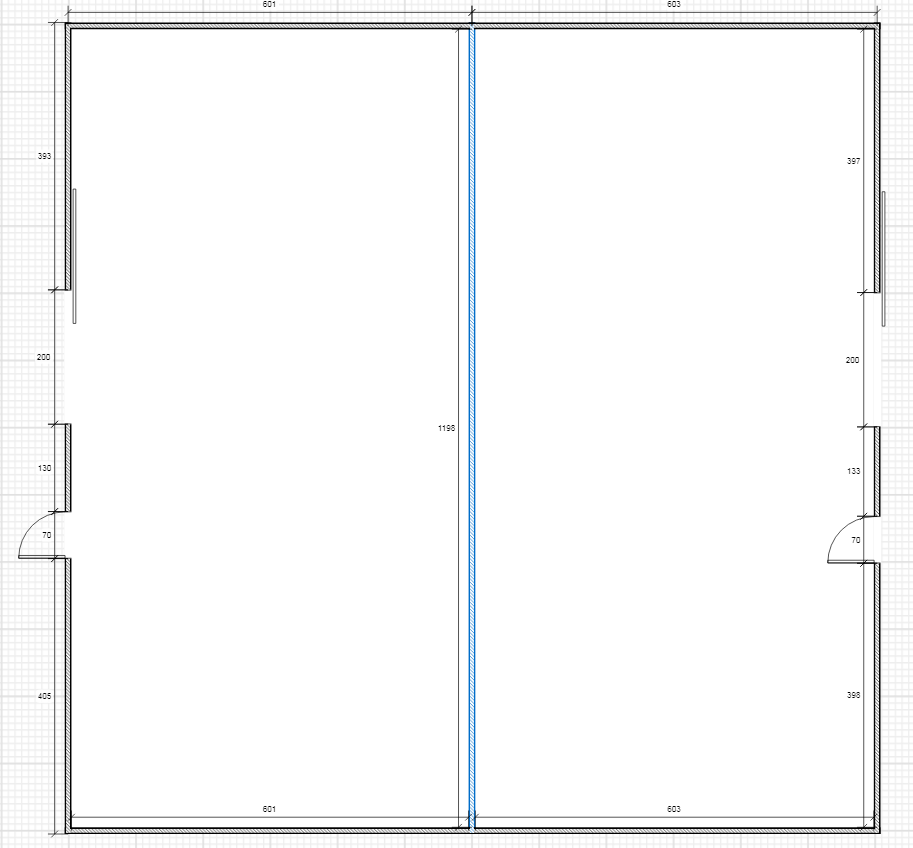
\includegraphics[scale=0.58]{./5-building.png}
 \caption{Поэтажный план здания №5}
\end{figure}
\end{document}